\section{Concurrency}\label{sec:concurrency}
The term concurrency is a general term for ways a computer system performs multiple tasks 'at the same time'. It covers the \textit{simulation} of multiple tasks running at the same time through process switching, as well as work done in parallel. To disambiguate, based on the definition:

\blockcquote{Bryant2016}{We use the term concurrency to refer to the general concept of a system with multiple, simultaneous activities, and the term parallelism to refer to the use of concurrency to make a system run faster.}

We infer that parallelism is a type of concurrency with the purpose to speed up the system, while concurrency in general may have purposes not related to speed.

Concurrency is a large and hardware dependant subject. To prevent falling into a concurrency rabbit hole, the limitations of the Arduino hardware in relation to concurrency, specifically the \gls{cpu}, is explored before concurrency in general. This is done because the project is, first and foremost, about programming language design - not concurrency.

\subsection{Arduino hardware}\label{subsec:arduinohardware}
The Arduino Uno board uses the ATmega328P microcontroller \cite{ArduinoUno}. The architecture of this microcontroller is a scalar single core processor, without hyperthreading(intel) or \gls{smt} (AMD) equivalents \cite{ATmega328P}.

Since there is only a single core, and that core does not contain any duplicate copies of CPU hardware (for multithreading), the only hardware parallelism on the Arduino Uno is instruction-level parallelism, and only to the level of up to 1 instruction per clock cycle (scalar). This is also handled directly by the \gls{cpu}, and does not impact the instruction set available to developers.


\begin{figure}[htb!]
    \centering
    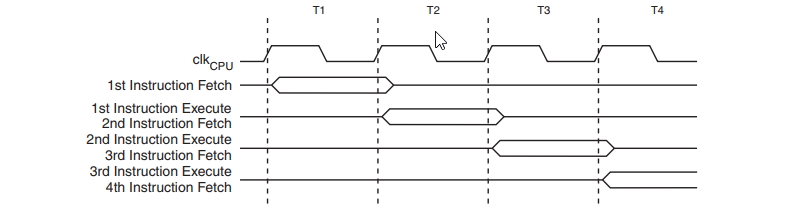
\includegraphics[width=\textwidth]{figures/Arduino_Pipeline.png}
    \caption{The parallel intruction fetches and intruction executions \cite{ATmega328P}}
    \label{fig:arduinopipeline}
\end{figure}


The Arduino is therefore a uniprocessor\cite{Bryant2016} - its architecture does not support parallel processing - and for the remainder of the report the term concurrency refers to: concurrency \textbf{without parallelism}.

\subsection{Models of concurrency}\label{subsec:modelsofcon}
Even unicore processors can support several models for concurrency at the application software level. This makes sense since most computers often has more processes running than it has \glspl{cpu}. This is done through interweaving instructions of different processes, which lets the \gls{cpu} appear to run multiple programs.

This interweaving is commonly handled through an \gls{os}, which manages the hardware resources \cite{Bryant2016}. However by default, the Arduino does not have an \gls{os}. It is still possible to achieve concurrency on an Arduino, but not without a scheduler, or scheduling, of some kind.

The scheduler is the part of the \gls{os} that handles the planning and switching of different tasks on the CPU within the system. However, an \gls{os} is not the only way to obtain scheduling behaviour. Several tutorials \todo{Insert citations to example links} demonstate different techniques to achieve concurrency on an Arduino, such as the use of the Arduino functions millis() and interrupt().

The milis() technique executes different pieces of code, depending on some programmer defined timeslices and comparisons between the current time and a previous time, while the interrupt() method uses the \gls{cpu} interrupt command to interrupt the \gls{cpu}, and restart it from another place in the code.

Both methods require the programmer to think deeply about how they wish for the program to execute, which gets complicated and potentially frustrating fast. In the case of the millis() method, a lot of variables may be required to execute the program correctly, which is hard track of.In the interrupt() case, it is a very low level command which might not work entirely as a novice or hobbyist expects.

It is also possible to install an \gls{os} on the Arduino, and obtain a scheduler (and other things) that way.

\subsection*{Deprecated at the moment}
% might be relevant to explain the concurrency models of an OS, to compare the choices.
This interweaving is commonly handled through an \gls{os}, which manages the hardware resources \cite{Bryant2016}. A few different approaches for interweaving processes are supported by most \glspl{os}: 

\subsubsection{Processes}
In this model the kernel, the portion of the \gls{os} code that resides in memory while the system is running, schedules and maintains each logical control flow, called a process. Each process has its own virtual address space, and therefore requires a mechanism for interprocess communication \cite{Bryant2016}.

\subsubsection{I/O multiplexing}
When an application explicitly schedules its own logical control flow, in the context of a single kernel process, you have I/O multiplexing. In the application, each logical control flow is modelled as a state machine, with the transitions defined and managed by the application code. Since this model is a single process, control flows share virtual address space \cite{Bryant2016}.

\subsubsection{Threads}
